\documentclass{article}
\usepackage{cite}
\usepackage{url}
\usepackage{graphicx}
\usepackage[utf8]{inputenc}
\usepackage[spanish,es-tabla]{babel}

\title{La reducción del número de piratas como causa del calentamiento global}
\author{Bobby Henderson}
\date{October 2019}

\begin{document}

\maketitle

\section{Resumen}

\begin{itemize}
    \item Url del Repositorio: \url{https://github.com/jorgechp/proyecto_final}
\end{itemize}

Se denomina calentamiento global al aumento de la temperatura en el Planeta Tierra así como a sus efectos. Si bien el calentamiento global es un fenómeno observado desde hace varias décadas, actualmente se ha convertido en un foco mediático así como en objeto de estudio desde diferentes campos de la ciencia. En este artículo, analizamos el fenómeno del descenso global del número de piratas y planteamos su inevitable relación con respecto al calentamiento global. Tras realizar diferentes pruebas de carácter empírico, encontramos que el número de piratas guarda una estrecha correlación y, por ende, causalidad, con respecto al aumento global de la temperatura en el planeta y con la victoria de Donald Trump como candidato a la presidencia de los Estados Unidos de América. 

\begin{itemize}
	\item Palabras clave: Piratas, calentamiento global, Donald Trump, mayonesa, temperatura.
\end{itemize}

\section{Introducción}
\subsection{Cambio climático}

Actualmente, el estudio del cambio climático, sus causas y los efectos de este, está requiriendo una cada vez mayor atención por parte de diferentes autores, centros de investigación y estados. Conocemos la relación existente entre calentamiento global y emisión de gases que producen el llamado \emph{Efecto Invernadero}. 

Sin embargo, aún hoy no se ha investigado de forma seria y rigurosa la aparentemente estrecha relación existente entre cambio climático y número de piratas. Esta línea de investigación defiende que el cambio climático está fuertemente causado por el descenso del número de piratas y que, conforme el número de piratas siga decreciendo, el calentamiento global seguirá aumentando y, en consecuencia, se agravarán los problemas generados por el calentamiento global.

En este artículo, analizamos diferentes factores que inciden en la repercusión que tienen los piratas sobre el calentamiento global y se estudia si estamos acercándonos a un punto de no retorno en el cual nunca más podremos ver surcar piratas en nuestros mares, y, por consiguiente, nunca más podremos beber agua en nuestras casas o regar nuestros campos.


\section{Estado del arte}
\subsection{Cambio climático}

En los dos últimos siglos, nuestro planeta ha experimentado un incremento gradual de la temperatura media. La observación de este fenómeno, así como de sus causas, se denomina \emph{Calentamiento Global}  \cite{mann_selin_2019, rahayuglobal}. El incremento de temperatura global se ha ido acelerando paulatinamente, siendo en la última década, de aproximadamente 0.93 grados \cite{alen}. 

A nivel social, existe una concienciación cada vez mayor sobre el cambio climático y sus efectos. No obstante, la opinión pública tiende a asumir conceptos erróneos sobre el Cambio climático. Por ejemplo, existen confusión a la hora de distinguir el agujero de la capa de ozono con el efecto invernadero, así como a utilizar indistintamente \emph{clima} y \emph{tiempo}\cite{bostrom}. Si bien es una posición considerada minoritaria, existen voces que niegan el cambio climático, especialmente en el ámbito de empresas que tienen intereses financieros en segmentos de la economía que tienen una incidencia medioambiental muy elevada \cite{astroturf}.

La comunidad académica se centra en los últimos años en el estudio del cambio climático y sus causas. En los últimos años, han cobrado relevancia tesis que identifican las emisiones de $CO^2$ como un factor significativo para explicar el fenómeno del aumento de la temperatura global \cite{whitmarsh2011}. En cualquier caso, la hipótesis de que el la acción humana tiene una gran repercusión en el medio ambiente hoy en día se encuentra, generalmente, aceptada.

\subsection{Piratería}
Se entiende por piratería al acto de cometer delitos de pillaje o violencia criminal contra barcos o zonas costeras \cite{pennell_2001}. Los primeros documentos que describen casos de piratería podemos encontrarlos en el siglo XIV cuando un grupo de navegantes, conocidos como los \emph{Pueblos del mar}, emprendieron ataques contra diferentes civilizaciones repartidas por el Mar Mediterráneo y el Mar Egéo y en zonas de importancia estratégica como el Estrecho de Gibraltar. No obstante, aunque sin esta denominación, la piratería ya era común en el Siglo II antes de Cristo \cite{lane2015}.

Los piratas tuvieron una importancia muy relevante a partir de la llegada de Cristobal Colón a América, donde las naciones occidentales experimentaron un crecimiento muy importante de sus flotas y se establecieron nuevas rutas comerciales por los Océanos Atlántico y Pacífico. Es también esta época cuando la relación entre estados y piratas gana complejidad: llegando los primeros a realizar pactos con los segundos para defender sus intereses o para boicotear comercial a sus adversarios. Especialmente relevante es el caso de Inglaterra, quien estableció fuertes relaciones con piratas para atacar intereses comerciales de la Corona de Castilla así como de otras potencias rivales \cite{hebb2016}.

Se denomina \emph{Edad de oro de la piratería} a diferentes periodos de la Edad Moderna en los que se asistió a un importante surgimiento de la piratería. Generalmente, se acepta que este periodo duró desde 1625 hasta 1795 \cite{little2010}. Tras esta edad de oro, la actividades de los piratas empezaron a descender paulatinamente. 


\begin{figure}[h]
    
\includegraphics[width=12cm]{jolly_roger.png}
    \caption{La \emph{Jolly Roger} fue la bandera utilizada por los piratas durante la Edad Moderna.}
    \centering
\end{figure}

Finalmente, durante el siglo XX, se hizo patente el descenso de la piratería a nivel global. Actualmente, aún existen actividades de piratas, especialmente en el Océano Índico \cite{gomez2013}.

\section{Hipótesis y método}

Tras el minucioso análisis del estado del arte realizado en el apartado anterior, solo podemos plantearnos la siguiente hipótesis:

\begin{enumerate}
    \item El descenso del número de piratas es la principal causa del cambio climático
\end{enumerate}

Para corroborarlo, se ha realizado un análisis sobre el descenso del número de piratas a lo largo de los últimos doscientos años así como el incremento progresivo de la temperatura global. Nuestra principal fuente de conocimiento al respecto ha sido \emph{Google Images}.

\section{Resultados}

Los resultados recogidos en este trabajo relacionan la evolución del calentamiento global con respecto al número de piratas que quedan vivos. Como se puede apreciar en la gráfica que se muestra a continuación, el descenso de piratas ha sido especialmente significativo durante el siglo XX si bien, siempre ha existido una tendencia a la baja.

Del mismo modo, podemos analizar el calentamiento globar desde desde el surgimiento de la Revolución Industrial, notando como la temperatura se ha ido incrementando de forma paulatina.


\begin{figure}
  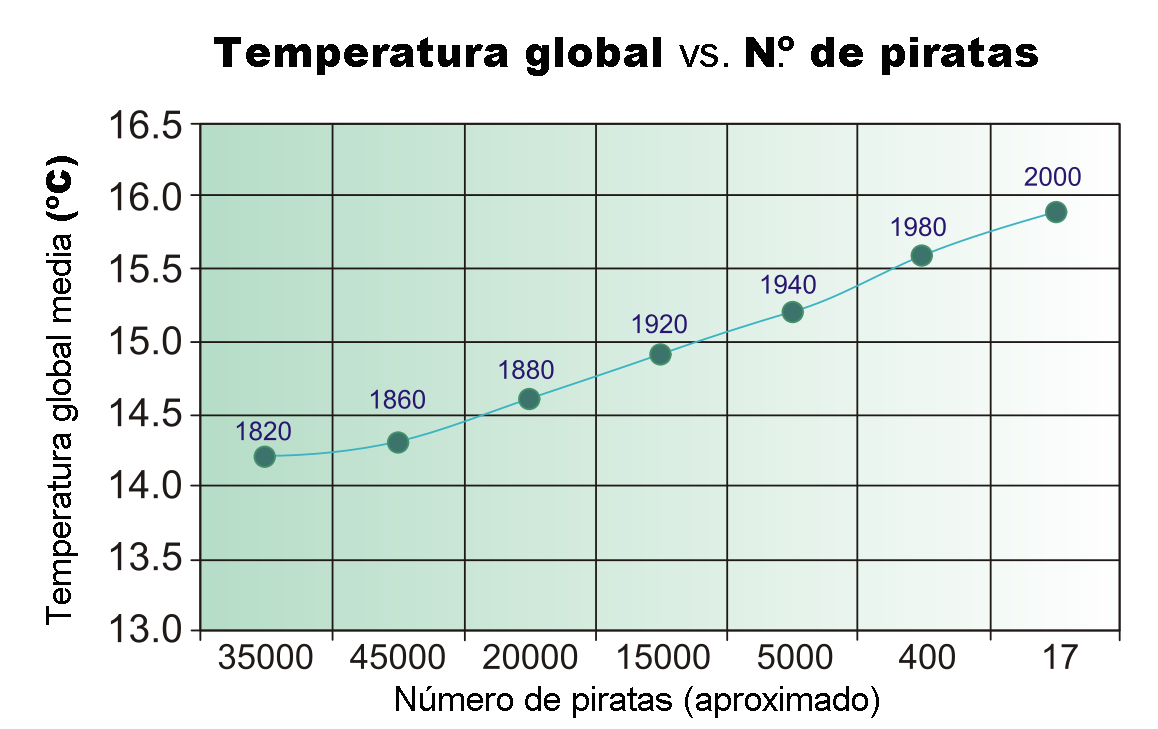
\includegraphics[width=\linewidth]{graph_1.png}
  \caption{Temperatura global vs descenso del número de piratas.}
  \label{fig:grafico_1}
\end{figure}



\begin{table}[h]
\centering
\begin{tabular}{|l|l|l|}
\hline
\multicolumn{1}{|c|}{\textbf{Año}} & \multicolumn{1}{c|}{\textbf{Temperatura global}} & \multicolumn{1}{c|}{\textbf{Número de piratas}} \\ \hline
1820                               & 14.2                                             & 35000                                           \\ \hline
1860                               & 14.3                                             & 45000                                           \\ \hline
1880                               & 14.6                                             & 20000                                           \\ \hline
1920                               & 14.9                                             & 15000                                           \\ \hline
1940                               & 15.3                                             & 5000                                            \\ \hline
1980                               & 15.6                                             & 400                                             \\ \hline
2000                               & 15.8                                             & 17                                              \\ \hline
\end{tabular}
\caption{Relación entre número de piratas y temperatura media global.}
\label{table:tabla_1}
\end{table}

Podemos expresar la relación entre el calentamiento global y el número de piratas en la tierra mediante la siguiente ecuación:

\begin{equation}
    Y = -3.395e-005\cdot X + 15.54 
\end{equation}


Donde:
\begin{itemize}
    \item Y representa la temperatura media global.
    \item X representa el número de piratas.
\end{itemize}

En la Tabla \ref{table:tabla_1} se aprecia de igual manera cómo se está produciendo un descenso en el número de piratas. Por otro lado, también podemos mostrar una gŕafica (ver figura \ref{fig:grafico_2}) con la relacion entre el número de películas en las que aparece Nicolas Cage con respecto al número de muertes de personas que han caído a piscinas.

\begin{figure}
  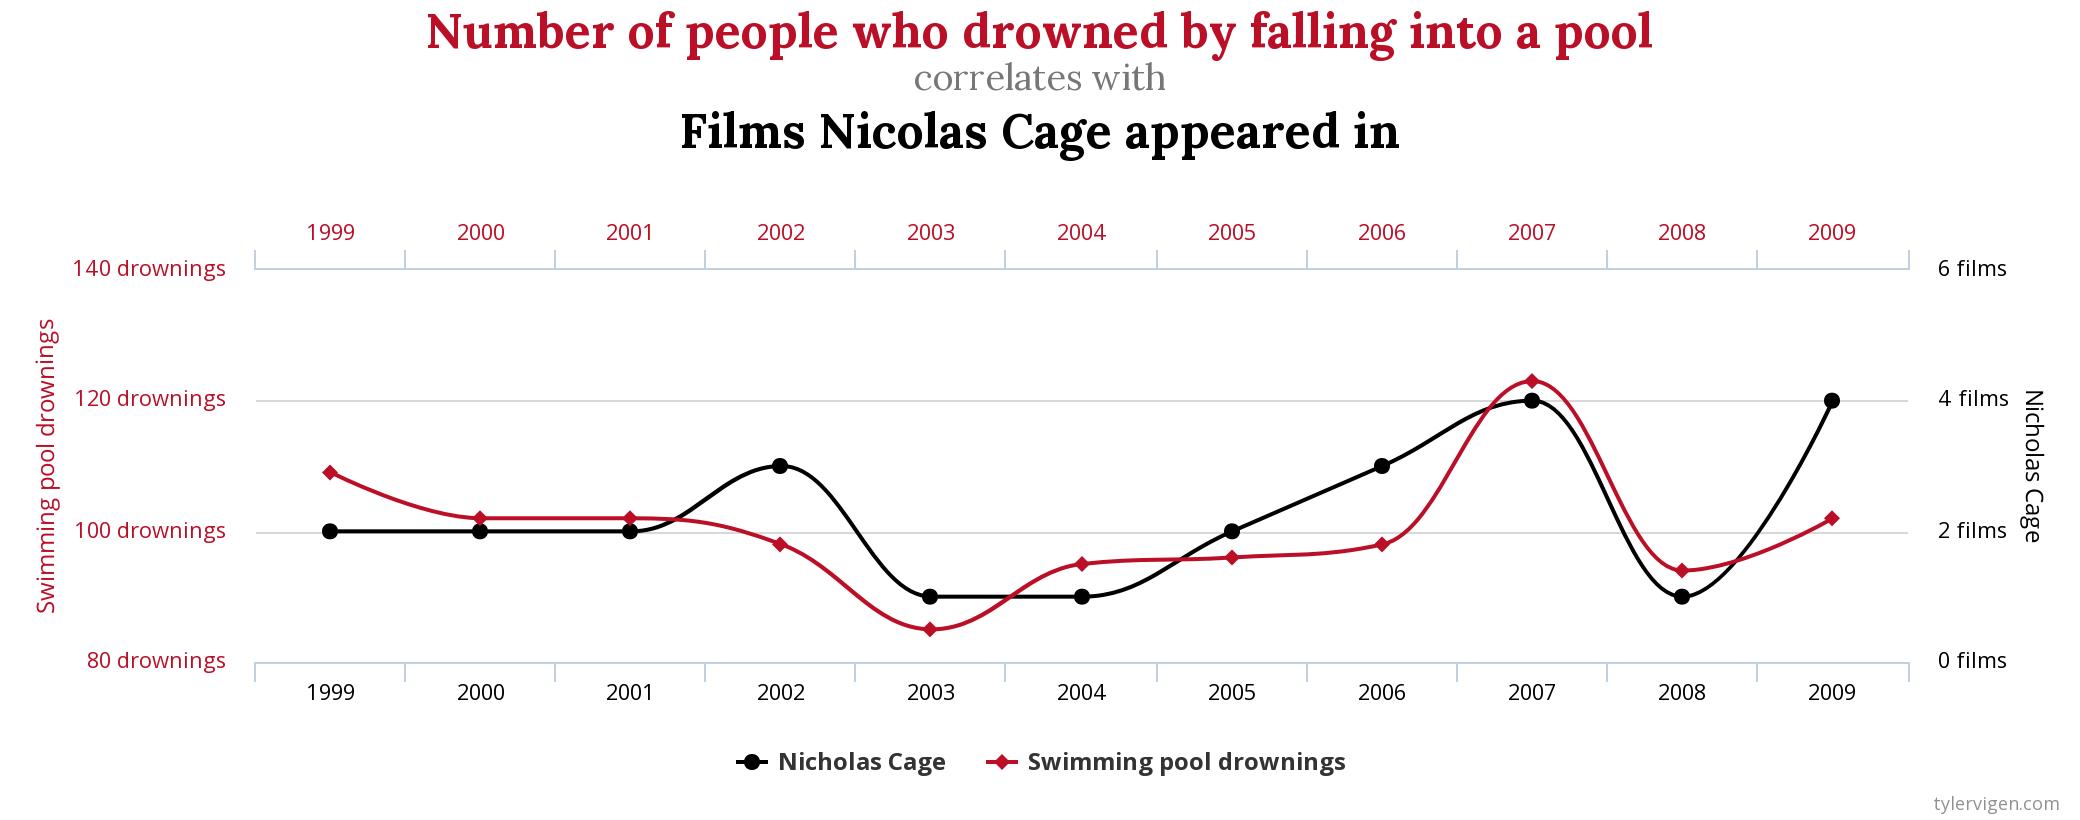
\includegraphics[width=\linewidth]{graph_2.png}
  \caption{Número de películas donde aparece Nicolas Cage vs número de ahogamientos por caída en piscina.}
  \label{fig:grafico_2}
\end{figure}




\section{Conclusiones}

Tras los resultados obtenidos en nuestro riguroso estudio, es inapelable concluir que el calentamiento global se debe única y exclusivamente al descenso del número de piratas sobre nuestros mares y océanos.




\bibliography{bibliography}{}
\bibliographystyle{plain}

\end{document}
